\subsection*{Implementation Architecture}

The XNAT platform is an integrated suite of software based on open source technologies and custom code. The software design is standard and expandable separating out client interfaces, middleware engines, and data archiving. This modular design eases development by having well formed boundaries, a tested core foundation, and debugging access to every area. An abstracted XNAT architecture is presented in \ref{fig:architecture} \cite{xnat}, with the redaction plug-in indicated in bold.

\begin{figure}[hbt]
       \center{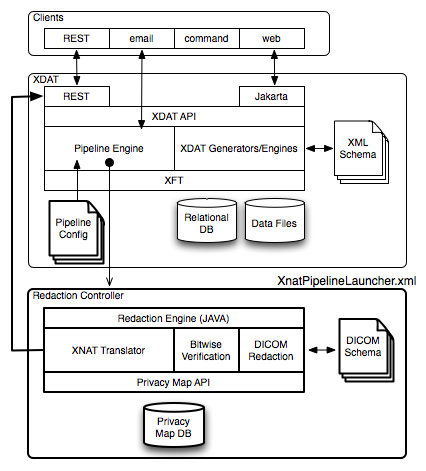
\includegraphics[scale=.7]{architecture_pipeline.png.png}}
        \caption{\label{fig:architecture} Preliminary architecture diagram (modifications in bold)}
\end{figure}
% Sept 11 AB - Changed pic to new architecture, PNG, no bounding box/export full size

The redaction effort can be divided logically and by software implementation into three primary components: (1) the redaction engine, (2) the privacy mapping database, and (3) the XNAT translator. The first two integrate into the XNAT pipeline facility\cite{xnatpipeline}, where the specification and configuration for the pipeline are defined in Extensible Markup Language (XML) files \cite{bray2000}. The XML documents are configuration files; which define how the pipeline works, and operates as a template for XNAT database and web presentation. The pipeline configuration and provided utility program enable the redaction process to be XNAT aware by providing feedback to the user via e-mail with problems or status updates.

The redaction engine is an expandable entry point and controller of the redaction tool, and by design has to start as a JAVA program. This is currently planned to encompass both the DICOM redaction procedure and the low-level bitwise verification mechanism, however final language choice and detailed design decisions will occur during development. 

The DICOM redaction component is based on in-depth knowledge of the DICOM file format and the conformance statements from the major MRI vendors. By parsing the DICOM file, a list of the name:value pairs can be extracted from the file itself. These defined duples identify PII, which can then be remapped to anonymized identifiers. This process of matching and replacement of name:value pairs enables the researcher to redact any DICOM field through the use of DICOM translation schemas. The shipping configuration will be tailored to HIPAA compliance, but the framework will be in place for any DICOM conversion. 

This remapping process is verified on the resultant DICOM image to ensure confidentiality of the original data. Digital forensics has pioneered the concept of ignoring the structure of files and file systems, opting instead to use low level bitwise datastream from disk and manually searching for information. This technique will be applied to DICOM files, searching for PII as search terms. This will be built on an open source data carving tool, such as scapel\cite{scapel}.

The anonymized identifiers and original data are stored in an encrypted privacy mapped database. This database is an integral part of the system, containing the link between the original images and their redacted counterparts. The API acts as a gatekeeper ensuring integrity of the databases by exposing a non-harmful subset of commands to the redaction engine and client application. The privacy map provides consistency between research subjects, ensuring the consistency of redacted ID to subject PII, preventing skew in statistical analysis due to duplication of data. This will be implemented as an additional database on top of the PostgreSQL instance already being utilized by XNAT. 

The last part of the redaction process is creation of new XNAT identifiers and transmission of the redacted data. The translator will communicate with XNAT through the HTTP REST interface provided \cite{fielding2000} and secure FTP where it will be uploaded to XNAT as new images, but with different metadata, where it will be processed as any incoming data. 

The proposed architecture is not complex, it is an extension to well conceived and executed system. The redaction design mimics that of XNAT itself; modular components, open source, simple to use, and simple to extend for future needs. 